Substituting
\begin{align}
 \vec{P}=\myvec{
-1\\
3
},
\vec{n}=\myvec{
3\\
-4
}, c=16
\end{align}
in 
	\eqref{eq:11/10/3/4/foot_of_perpendicular},
the desired foot of the perpendicular is then given by 
\begin{align}
\myvec{4&3\\3&-4}\vec{Q}=\myvec{\myvec{4&3}\myvec{-1\\3}\\16}
=\myvec{5\\16}  
\\
\implies
  \myvec{
   4 &  3  & 5\\
   3 & -4  & 16} 
  \xleftrightarrow[]{R_2=R_2-\frac{3}{4}R_1}
  \myvec{
  4 & 3 & 5\\
  0 & \frac{-25}{4} & \frac{49}{4}} 
\\
  \xleftrightarrow{R_2=\frac{-4}{25}}
  \myvec{
  4 & 3 & 5\\
  0 & 1 & \frac{-49}{25}}
  \xleftrightarrow{R_1=\frac{1}{4}R_1}
  \myvec{
  1 & \frac{3}{4} & \frac{5}{4}\\[1ex]
  0 & 1 & \frac{-49}{25}}
\\
  \xleftrightarrow{R_1=R_1-\frac{3}{4}R_2}
  \myvec{
  1 & 0 & \frac{68}{25}\\[1ex]
  0 & 1 & \frac{-49}{25}}          
\implies \vec{Q}=\myvec{
\frac{68}{25}\\[1ex]
\frac{-49}{25}
}
\end{align}
See 
\figref{fig:chapters/11/10/3/14/Fig}.
\begin{figure}[H]
	\begin{center} 
	    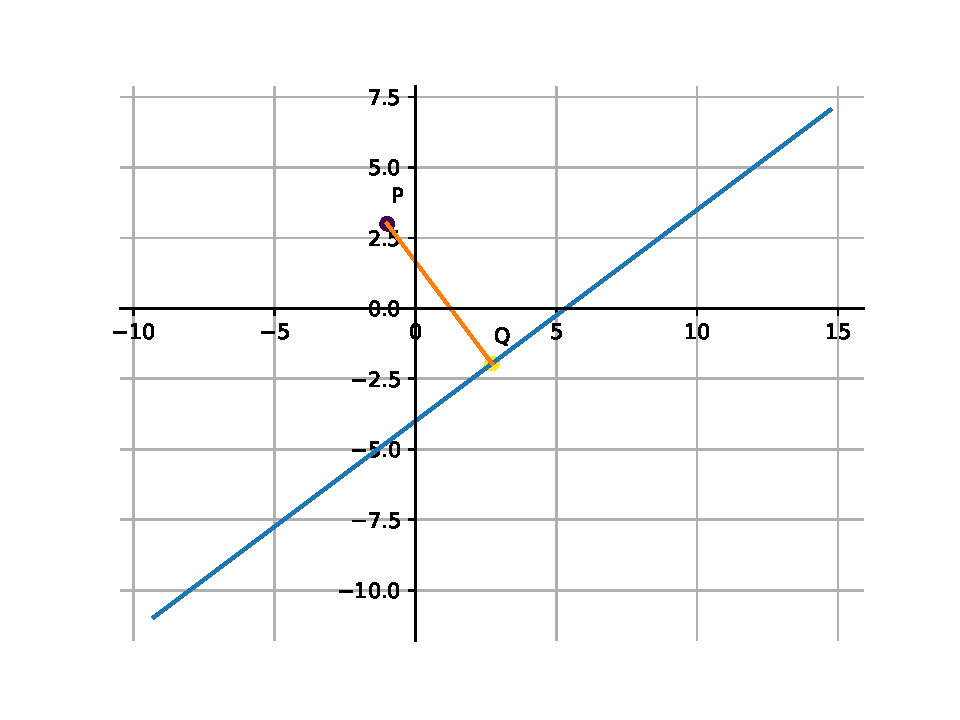
\includegraphics[width=0.75\columnwidth]{chapters/11/10/3/14/figs/fig.pdf}
	\end{center}
\caption{}
\label{fig:chapters/11/10/3/14/Fig}
\end{figure}
